% Author : Alexandre Corizzi
% Creation: 10/09/2020
% Update: 21/02/2023 

\pdfminorversion=7
\documentclass[a4paper,11pt,notitlepage]{article}
\usepackage{sectsty}
\usepackage[hidelinks]{hyperref}
\usepackage{stmaryrd}
\usepackage{float}
\usepackage{placeins}
% \usepackage{hyperref}

\hypersetup{
  colorlinks   = true,      % Colours links instead of ugly boxes
  urlcolor     = RoyalBlue, % Colour for external hyperlinks
  linkcolor    = NavyBlue,  % Colour of internal links
  citecolor   = red         % Colour of citations
}

\sectionfont{\color{astral}}
\subsectionfont{\color{astral}}
\subsubsectionfont{\color{astral}}
\usepackage[
  top=4.6cm,
  bottom=2cm,
  left =1.8cm,
  right=1.8cm,
  headheight=94pt, 
  includehead,
  includefoot,
  heightrounded, % to avoid spurious underfull messages
]{geometry} 

\addtolength{\textheight}{90pt}
\addtolength{\topmargin}{-90pt}

% Smiley clock : 
\usepackage[clock]{ifsym}
% Tilde :
\usepackage{textcomp} 

% Listings
\usepackage[utf8]{inputenc}
\usepackage{listings, color, upquote}
\usepackage[dvipsnames]{xcolor}
\definecolor{astral}{RGB}{46,116,181}

% Figures
\usepackage{subfigure}
\usepackage{graphicx}
\usepackage{url}

% Tableaux 
\usepackage{tabularx}
\usepackage{multirow}
% Rotating table
\usepackage{rotating} 

% Header 
\usepackage{fancyhdr}
\pagestyle{fancy}

% Listing Bash
\lstset{
                     numbers          = none,           
                     basicstyle       = \ttfamily\normalsize,
                     numbers          = none,           
                     frame            = single,
                     backgroundcolor  = \color{gray!10},
                     commentstyle     = \color{MidnightBlue},
                     keywordstyle     = \color{RedViolet},
                     stringstyle      = \color{red},
                     emphstyle        = \color{Bittersweet},
                     rulecolor        = \color{black},
                     emph             = {for, in},
                     keepspaces       = true,
                     showspaces       = false,
                     showstringspaces = false,         
                     showtabs         = false,                 
                     tabsize          = 4,                      
                     title            = \lstname,
					 aboveskip        = 0pt,
					 belowskip        = 10pt
}

% Listing Output
\lstdefinelanguage{commandline}{
    sensitive=false
} 
\lstdefinestyle{output}{
					 language         = commandline,
					 numbers          = left,
					 xleftmargin      = 2em,
					 framexleftmargin = 2em
}


%==============================================================================%
%                              Header/Footer                                   %
%==============================================================================%
% Params of the doc :
\newcommand{\reference}{HYPERNETS\_D4.7\_User\_Manual\_V\numVersion}
\newcommand{\numVersion}{2.1}
\newcommand{\titleDoc}{D4.7 User Manual}
% Header
\fancyhf{} % sets both header and footer to nothing
\renewcommand{\headrulewidth}{0pt}
\fancyhead[c]{
\begin{center}
\begin{tabularx}{\textwidth}{|c|X|l|}
    \hline
    \multirow{3}{*} {
\includegraphics[scale=.080]{logoHypernets.png}}            
     & Reference    &     \reference            \\
     \cline{2-3}
    \multirow{3}{*} & Version  &  \numVersion   \\
     \cline{2-3}
    \multirow{3}{*} & Date     &  \today        \\
    \hline
\end{tabularx}
\end{center}}
% Footer
\fancyfoot[l]{Confidential \copyright HYPERNETS Consortium (RBINS, TARTU, SU, 
CNR, NPL, GFZ, CONICET)}
% Pagination
\fancyfoot[r]{\thepage}

%==============================================================================%
% Command for "clock + time required" displaying
%==============================================================================%
\newcommand{\timeclock}[2]{
	\vspace{1pt}
	\textbf{\showclock{#1}{#2}\hspace{1pt} Required time:}
	\ifx0#1 \textbf{#2 min}
	\else   \textbf{#1 h #2}
	\fi}

%==============================================================================%
% Command to round angles on pictures
% src: https://subscription.packtpub.com/book/hardware-&-creative/9781784395148/4/ch04lvl1sec45/cutting-an-image-to-get-rounded-corners
%==============================================================================%
\usepackage{tikz}
\newsavebox{\picbox}
\newcommand{\cutpic}[3]{
	\savebox{\picbox}{\includegraphics[width=#2]{#3}}
	\tikz\node [draw, rounded corners=#1, 
	line width=1pt,
	color=astral, 
	minimum width=\wd\picbox, 
	minimum height=\ht\picbox, 
	path picture={\node at (path picture bounding box.center)
	{\usebox{\picbox}};}] {};}
%==============================================================================%
% usage: \cutpic{1cm}{\textwidth}{image.jpg}
%==============================================================================%



%==============================================================================%
%                               Début du document                              %
%==============================================================================%
% Chapter Selection:
% \includeonly{src/mounting_guide, src/linux_installation}
% \includeonly{src/hypernets_tools, src/first_tests, src/old_version_manual}
% \includeonly{src/first_tests, src/annex_config_files}
%==============================================================================%

\begin{document}
\hypersetup{pageanchor=false}
\begin{titlepage}
\thispagestyle{fancy}
\vspace*{8mm}
\begin{center}
    \begin{tabularx}{\textwidth}{c}
        
\includegraphics[scale=.23]{logoHypernets.png}
        \vspace{2mm} \\
        \Large{\textbf{\titleDoc}} \\
        \Large{\textbf{Version \numVersion}} \\
        \Large{\textbf{\today}}
    \end{tabularx}
\end{center}
\end{titlepage}
%==============================================================================%
\setcounter{page}{2}
\noindent Version History
\vspace{8pt}
\newline
\begin{tabularx}{\textwidth}{|l|l|X|l|}
\hline
\textbf{Version} & \textbf{Date}     & \textbf{Description} & \textbf{Author} \\ \hline
            0.1  & September 10, 2020     & First Draft & Alexandre Corizzi   \\ \hline
            0.2  & September 16, 2020     & Feedback from Clémence Goyens & 
			Alexandre Corizzi \\ \hline
            0.3  & September 22, 2020     & Notes from Clémence Goyens    
			& Alexandre Corizzi \\ \hline
            0.4  & September 24, 2020     & Comments from Javier Concha 
			& Alexandre Corizzi \\ \hline
			0.5  & September 29, 2020     & Draft Notebook Tests Section
			& Clémence Goyens \\ \hline
			0.5b  & October 1, 2020       &  Pan/Tilt RS485 Config + FTP Link 
			Correction & Alexandre Corizzi \\ \hline
			0.5c  & October 1, 2020       &  Feedback from Joel Kuusk
			& Alexandre Corizzi \\ \hline
			1.0a  & March 29, 2021   & Update with new software
			& Alexandre Corizzi \\ \hline
			1.0b  & May 27, 2021     & Timezone and other minor changes
			& Alexandre Corizzi \\ \hline
			1.0c  & June 9, 2021     & Add Yoctopuce annex
			& Alexandre Corizzi \\ \hline
			1.1a  & July 15, 2021    & Switch to Beta Version \& Yoctopuce Update
			& Alexandre Corizzi \\ \hline
			1.1b  & July 16, 2021    & Comments by David Doxaran  
			& Alexandre Corizzi \\ \hline
			1.1c  & July 28, 2021    & Comments by Joel Kuusk
			& Alexandre Corizzi \\ \hline
			2.0  & February 21, 2023    & Add Mounting Illustrations \& Debian
			& Alexandre Corizzi \\ \hline
			2.1  & April 21, 2023    & Update GUI screenshots, metadata configs
			& Alexandre Corizzi \\ \hline
			2.2  & July 17, 2023    & Update Debian section 
			& Alexandre Corizzi \\ \hline
			2.2b  & November 23, 2023  & Disambiguation of DIO wiring
			& Ana I. Dogliotti \\ \hline

\end{tabularx}
\newpage
%==============================================================================%
% \hypersetup{linkcolor=true}
\tableofcontents
\clearpage

%==============================================================================%
%                             Première page                                    %
%==============================================================================%
\section{Executive summary}

This document aims to guide step by step the user to perform the installation of
a Hypernets System. Firstly, a basic illustrated guide to assemble the
different mechanical and electronic parts of the system will take place.
Secondly, a tutorial about the installation of the a Linux operating system will be 
described. This, including both Manjaro and Debian Linux on the embedded computer 
(rugged PC). In third place, the basic set-up and some essential tests to move the 
pan-tilt - motor part of the system - and making some Hypstar Radiometer measurements 
will be provided. Finally, a procedure to make automatic measurements at 
arbitrary times - the autonomous mode - will be described.

\newpage

%==============================================================================%
%==============================================================================%
% Mounting part
%==============================================================================%

\section{Mounting Guide}

\subsection{Material List}

\begin{table}[!h]
	\begin{tabularx}{\textwidth} {
			| >{\hsize=.15\hsize}X
			| >{\hsize=.55\hsize}X
			| >{\hsize=.30\hsize}X | }
		\hline
		\textbf{Provider} & \textbf{Designation} & \\
		\hline
		\hline
		Tartu & Pan-tilt, Instrument \& Validation Module 
		& Right part of the Figure \ref{fig:hypstarYocto}
		\\ \hline
	  	& RS485 Serial Board Converter 
		& Green Card in the Figure \ref{fig:hypstarYocto}
		\\ \hline
		& Alignement Tool & Figure \ref{fig:alignement}
		\\ \hline
		& Anti-Dust Cap & Figure \ref{fig:antiDust}
		\\ \hline
		& Mechanical Part & Metal parts in the Figure \ref{fig:hypstarYocto}
		\\ \hline

		Studiel & Main Box & Figure  \ref{fig:StudielBoxMain}
		\\ \hline
		& Ancillary Box & Figure \ref{fig:StudielBoxAnci}
		\\ \hline
		& Junction Box & Figure \ref{fig:StudielJunction} 
		\\ \hline
		& 1 Green Samtec Cable (Main box -- Junction box) & Figure \ref{fig:StudielCable}
		\\ \hline
		& 1 Orange Samtec Cable (Main box -- Ancillary box) & Figure \ref{fig:StudielCable}
		\\ \hline
		& 2 Yellow Samtec Cables (Webcams) &
		\\ \hline
		& 1 Blue Samtec Cable (Power System -- Main box) & Figure \ref{fig:StudielCable}
		\\ \hline
		& 2 Ray tech Rapid Joint &
		\\ \hline
		Yoctopuce & Yocto-Pictor
		& Figure \ref{fig:yoctoDissas}
		\\ \hline
		N/A & Rugged PC Cincoze
		& Left part of the Figure \ref{fig:hypstarYocto}
		\\ \hline
		& Power system &
		\\ \hline
		& 2 Webcams Wi-Fi TVIP ABUS 62561 &
		\\ \hline
	\end{tabularx}
\end{table}

\clearpage



\begin{figure}[!ht]
	\centering
		\cutpic{5pt}{0.8\textwidth}{images/mount/IMG_9781.JPG}
		\caption{Yoctopuce, Rugged PC and Hypstar \& Validation Module}
		\label{fig:hypstarYocto}
\end{figure}

\begin{figure}[!h]
	\centering
	\begin{minipage}[b]{.8\textwidth}
		\cutpic{5pt}{\textwidth}{images/mount/IMG_9797.JPG}
		\caption{Studiel Cables}
		\label{fig:StudielCable}
	\end{minipage}
\end{figure}


\begin{figure}[!ht]
  \centering
  \begin{minipage}[b]{0.49\textwidth}
	  \cutpic{5pt}{\linewidth}{images/mount/IMG_9800.JPG}
	  \vspace{-20pt}
	  \caption{The Studiel main Box}
	\label{fig:StudielBoxMain}
  \end{minipage}
  \hfill
  \begin{minipage}[b]{0.49\textwidth}
	  \cutpic{5pt}{\linewidth}{images/mount/IMG_9788.JPG}
	  \vspace{-20pt}
	  \caption{The Studiel Ancillory Box}
	\label{fig:StudielBoxAnci}
  \end{minipage}
\end{figure}
\vspace{40pt}
\begin{figure}[!ht]
	\centering
	\begin{minipage}[b]{\textwidth}
		\cutpic{5pt}{\linewidth}{images/mount/IMG_9791.JPG}
		\vspace{-20pt}
		\caption{Studiel Junction Box}
		\label{fig:StudielJunction}
	\end{minipage}
\end{figure}
\vspace{-10pt}
\noindent \textcolor{red}{Please note that the mechanical mount for pan-tilt
and the powering system are not supported by this guide.}

\newpage
\clearpage

\subsection{Flip the metal piece on the top of the  instrument}
\timeclock{0}{10}

\vspace{10pt}
\noindent For shipping reasons -- size of the package, avoiding shipping damages -- 
the Hypstar Radiometer \& the Validation Module are shipped with the 
top metal wing mounted in the wrong way. First, fix the pan-tilt on your
mechanical mount. Unscrew the 4 screws (labelled in red on \ref{pic:instrum1})
and invert the direction of the wing like showed in the following pictures.

\vspace{10pt}
\noindent\textbf{\underline{Material List}:}
\begin{itemize}
	\item Allen key
\end{itemize}


\begin{figure}[!ht]
	\centering
	\begin{tikzpicture}
		\begin{scope}
			\node[anchor=center,inner sep=0] (image) at (0,0)
			{\cutpic{5pt}{\linewidth}{images/mount/IMG_9842.JPG}};
			\draw[red,ultra thick,rounded corners] (-5.1,3.6) rectangle ++(0.6,0.6);
			\draw[red,ultra thick,rounded corners] (-3.5,3.2) rectangle ++(0.6,0.6);
			\draw[red,ultra thick,rounded corners] (-5.4,2.55) rectangle ++(0.6,0.6);
			\draw[red,ultra thick,rounded corners] (-3.8,2.12) rectangle ++(0.6,0.6);
		\end{scope}
	\end{tikzpicture}
	\vspace{-20pt}
	\caption{Flip metal piece 1/3}
	\label{pic:instrum1}
\end{figure}

\begin{figure}[!ht]
	\centering
	\begin{minipage}{.8\textwidth}
		\cutpic{5pt}{\linewidth}{images/mount/IMG_9847.JPG}
		\vspace{-20pt}
		\caption{Flip metal piece 2/3}
		\label{pic:instrum2}
	\end{minipage}

	\vspace{30pt}

	\begin{minipage}{.8\textwidth}
		\cutpic{5pt}{\linewidth}{images/mount/IMG_9851.JPG}
		\vspace{-20pt}
		\caption{Flip metal piece 3/3}
		\label{pic:instrum3}
	\end{minipage}
\end{figure}


\newpage
\clearpage

\subsection{The Inside of the Studiel Box}
\timeclock{0}{30}
\vspace{10pt}

\noindent\textbf{\underline{Material List}:}
\begin{itemize}
	\item Allen key 2 and 5, Plate key 7
	\item Screw drivers (flat/slotted and cross slot) 
	\item Cutting plier
\end{itemize}

\subsubsection{Yocto-Pictor - Dissasembling \& Light Sensor}

\underline{Instructions}:

\begin{enumerate}
	\item Unscrew the four screws at the top of the Yocto-Pictor
	\item Split the Yoctopuce in two pieces (see figure \ref{fig:yoctoDissas})
	\item Cut the light sensor of the ground floor
	\item Fix it and plug it in the Studiel ancillary box (see figure
		\ref{fig:lightSensor})
\end{enumerate}
\textcolor{red}{Warning: make sure to correctly cut the PCB track of the light 
sensor before pulling it; there is a risk of ripping it of.}

\begin{figure}[!ht]
  \centering
  \begin{minipage}[b]{0.49\textwidth}
	  \cutpic{5pt}{\linewidth}{images/mount/IMG_9815.JPG}
	  \caption{Dissasembling the Yocto-Pictor}
	\label{fig:yoctoDissas}
  \end{minipage}
  \hfill
  \begin{minipage}[b]{0.49\textwidth}
	  \cutpic{5pt}{\linewidth}{images/mount/IMG_9819.JPG}
	  \caption{Placement of the Light Sensor}
	\label{fig:lightSensor}
  \end{minipage}
\end{figure}

\clearpage
\subsubsection{Yocto-Pictor - Reassembling in the Box}

\underline{Instructions}:
\begin{enumerate}
	\item Place the Yocto-Pictor ground floor with relays on the top 
		and the 4 screw tubes (figure \ref{fig:yoctoBottom})
	\item Plug the bottom-top bridge and add carefully the top floor 
		and fix it with screws (figure \ref{fig:yoctoTop})
	\item Fix and connect the GPS antenna; then follow the wiring Table \ref{table:yoctoWire}
\end{enumerate}

\begin{figure}[!ht]
  \centering
  \begin{minipage}[b]{0.49\textwidth}
	  \cutpic{5pt}{\linewidth}{images/mount/IMG_9828.JPG}
	  \caption{Fixing the bottom part}
	\label{fig:yoctoBottom}
  \end{minipage}
  \hfill
  \begin{minipage}[b]{0.49\textwidth}
	  \cutpic{5pt}{\linewidth}{images/mount/IMG_9830.JPG}
	  \caption{Fixing the top part}
	\label{fig:yoctoTop}
  \end{minipage}
\end{figure}


 \begin{table}[h]
	\begin{tabularx}{\textwidth} {| >{\hsize=.30\hsize}X| >{\hsize=.70\hsize}X| }
		\hline
		\textbf{Yocto-Pictor Pinouts} & \textbf{Studiel Box Connectors} \\
		\hline
		\hline
		Relay 1 & PC  (Rugged PC power) \\ \hline
		Relay 2 & PT  (Pan tilt) \\ \hline
		Relay 3 & MM  (Measurement Module) \\ \hline
		Relay 4 & RS  (Rain Sensor) \\ \hline
		Relay 5 & WC1 (Webcam 1) \\ \hline
		Relay 6 & WC2 (Webcam 2) \\ \hline
		Main Power &  YP (Studiel Box Connector) \\ \hline
		Light Sensor Connector & Dedicated tablecloth USB  \\ \hline
		USB config Port & USB-B Micro cable \\ \hline
	\end{tabularx}
	\caption{Wiring table for the Yocto-Pictor}
	 \label{table:yoctoWire}
\end{table}

\clearpage
\subsubsection{Rugged PC and Serial Board Converter fixing}

\underline{Instructions}:
\begin{enumerate}
	\item Attach the fixation support provided with the rugged PC, the grids upwards 
		(see the Figure \ref{fig:ruggedPCfix})
	\item Unscrew the four srews (shown on the Figure
		\ref{fig:StudielBoxRuggedPCemplacement})
	\item Fix the rugged PC ;  the side with DIO and the four serial ports must
		be toward the top of the Studiel Box
	\item Attach the serial board Converter and plug the brown cable in the
		slot A, the red cable in the slot B (Figure \ref{fig:serialBoard})
\end{enumerate}

\begin{figure}[!ht]
  \centering
  \begin{minipage}[b]{0.49\textwidth}
	  \cutpic{5pt}{\linewidth}{images/mount/IMG_9802.JPG}
	  \caption{Rugged PC - Fixation System}
	\label{fig:ruggedPCfix}
  \end{minipage}
  \hfill
  \begin{minipage}[b]{0.49\textwidth}
	  \cutpic{5pt}{\linewidth}{images/mount/IMG_9804.JPG}
	  \caption{Area for the Rugged PC in the Box}
	\label{fig:StudielBoxRuggedPCemplacement}
  \end{minipage}
\end{figure}


\begin{figure}[!ht]
  \centering
  \begin{minipage}[b]{0.75\textwidth}
	  \cutpic{5pt}{\linewidth}{images/mount/IMG_9832.JPG}
	  \vspace{-20pt}
	  \caption{Global view of the inside}
	\label{label}
  \end{minipage}
  \hfill
  \begin{minipage}[b]{0.24\textwidth}
	  \cutpic{5pt}{\linewidth}{images/mount/IMG_9838.JPG}
	  \caption{Serial Board Converter}
	\label{fig:serialBoard}
  \end{minipage}
\end{figure}

\noindent Now, you should have connectors pending next to their rugged PC pinouts that 
you can plug:
\begin{itemize}
	\item Connect the two DIO terminals as shown on the Figure
		\ref{fig:DIOwiring}
	\item Connect the RS485 wire (the one of the top) to the COM1
	\item Connect the power supply and the Ethernet connector
	\item Connect the USB cable for RS485 converter (HYPSTAR – Rugged PC connection)
	\item Connect the USB cable for Yocto-Pictor 
\end{itemize}

\vspace{20pt}
\begin{figure}[!ht]
  \centering
  \begin{minipage}[b]{0.49\textwidth}
	  \cutpic{5pt}{\linewidth}{images/mount/IMG_9855.JPG}
	  \vspace{-10pt}
	  \caption{Fixing the Junction Box}
	\label{fig:fixJunction}
  \end{minipage}
  \hfill
  \begin{minipage}[b]{0.49\textwidth}
	  \cutpic{5pt}{\linewidth}{images/mount/DIO_connection.png}
	  \vspace{-10pt}
	  \caption{Wiring the DIO}
	\label{fig:DIOwiring}
  \end{minipage}



\end{figure}

\noindent Unscrew the top of the Junction Box and fix it on the top of the pan-tilt
using the provided srews (see Figure \ref{fig:fixJunction}).

% Fix the GPS on the metal holder (stick the side where MOLEX is written).
% Fix the metal holder along the WIFI antenna.
% Take the WIFI and GPS antenna of the Yoctopictor
% Connect the GPS and WIFI antennas of the Yoctopuce
% Fix antennas (use the two small once)
% insert it into the Studiel main box

\clearpage
\subsection{Finalization}


\begin{figure}[!th]
	\centering
	\begin{minipage}[h]{0.6\textwidth}
		\vspace{-7cm}
		\underline{Instructions}:
		\begin{enumerate}
			\item Carefully remove the Alignement Tool (Figure \ref{fig:alignement})
			\item Place the anti-dust device (Figure \ref{fig:antiDust})
			\item Carefully respecting the color code, connect the cables
			\item Make sure the rugged PC switch is on \textit{AT}
			\item Close the box
		\end{enumerate}
	\end{minipage}
	\begin{minipage}[b]{0.3\textwidth}
		\cutpic{5pt}{\linewidth}{images/mount/IMG_9878.JPG}
		\vspace{-20pt}
		\caption{Remove the \textit{Alignement Tool}}
		\label{fig:alignement}
	\end{minipage}
\end{figure}


\begin{figure}[!ht]
	\centering
	\begin{minipage}[b]{0.30\textwidth}
		\cutpic{5pt}{\linewidth}{images/mount/IMG_9875.JPG}
		\vspace{-20pt}
		\caption{Put the anti-dust cap}
		\label{fig:antiDust}
	\end{minipage}
	\hfill
	\begin{minipage}[b]{0.65\textwidth}
		\cutpic{5pt}{\linewidth}{images/mount/IMG_9861.JPG}
		\vspace{-20pt}
		\caption{Fixing the cables}
		\label{fig:fixCables}
	\end{minipage}
\end{figure}

\begin{figure}[!ht]
  \begin{minipage}[b]{\textwidth}
	  \cutpic{5pt}{\linewidth}{images/mount/IMG_9869.JPG}
	  \caption{Overall Installation}
	\label{label}
  \end{minipage}
\end{figure}

\section{Installing a Linux Distibution}


\noindent\timeclock{1}{30}
\vspace{10pt}

This part aims to install a fresh linux system on the rugged PC. Most of the first
tests have been performed with \textit{Manjaro} Linux. However, any UNIX system could 
replace this distribution. We also have experimented few updating issue with
Manjaro as it is a \textit{rolling release distribution}. Hence the last version of 
the software has been tested with \textit{Debian} that might be the prefered
solution.

\vspace{10pt}
\noindent\textbf{\underline{Material List}:}
\begin{enumerate}
		\item Rugged PC Cincoze
		\item USB Stick up to 2GB
		\item Internet connection
		\item Screen, keyboard, and mouse
\end{enumerate}

\subsection{Debian Linux System}
\subsubsection{Creating an Installation USB of Debian Linux}
\par Alternatively you can use a Debian System, visit this 
\href{https://cdimage.debian.org/debian-cd/current/amd64/iso-cd/}{link}
and download those two files:
\vspace{-10pt}
\begin{lstlisting}
debian-11.7.0-amd64-netinst.iso
SHA256SUMS
\end{lstlisting}
Check-up the integrity of your downloaded file with:
\vspace{-10pt}
\begin{lstlisting}
sha512sum -c SHA512SUMS.txt
debian-11.7.0-amd64-netinst.iso: Success
\end{lstlisting}
The next step is to burn the image with:
\vspace{-11pt}
\begin{lstlisting}
umount /dev/sdX*
sudo dd if=/path/to/debian.iso of=/dev/sdX status="progress"
(replace sdX with the ID of your usb stick)
\end{lstlisting}
\vspace{6pt}
\textbf{\textcolor{red}{Double check your device name before writing onto
it (please refer to the equivalent \ref{usbLiveCreation} in the Manjaro
section)}}.

\subsubsection{Indicative settings for the Installation}

\begin{enumerate}
	\item Boot on the USB stick (see Annex \ref{annex:bios} to configure the 
		BIOS)
	\item Choose the \textit{Graphical Install} and the language
		\textit{English}
	\item Set \textit{United Kingdom} as  location and select your keyboard mapping
	\item Configure a Network connection for the installation
	\item Set up  machine name, user and root passwords
	\item Force UEFI installation: \textit{yes} 
	\item Select the \textit{guided partioning} with all files in one partition (recommended)
	\item Participate in the package usage survey: \textit{no}
	\item \textcolor{red}{Select the \textbf{Xfce} server X} and add
		\textit{standard system utilities}
\end{enumerate}
\vspace{1pt}
\noindent Once done, remove the USB key stick and reboot. You should see a
prompt asking you the password you previously setted-up. 
Open a terminal \textit{(ctrl + alt + t)} and type the following commands:
\begin{lstlisting}
rmdir Music/ Pictures/ Videos/ Public/ Templates/
su
<password>
/usr/sbin/usermod -aG sudo <username>
/usr/sbin/usermod -aG adm <username>
\end{lstlisting}
Logout, login and install git with: 
\begin{lstlisting}
sudo apt install git
\end{lstlisting}


\section{Hypernets Tools}

\subsection{Presentation}
\par \textit{hypernets\_tools} is the software developped for the Hypernets System.
It consists in a \textit{Git} repository, it is mainly developped with Bash and
Python (3.7+) languages. It is fully compatible with any UNIX system which
inclues \textit{apt} or \textit{pacman} and a functionnal \textit{systemd}
installation. It is also dependent on the \textit{libhypstar}, the \textit{driver} 
library of the Hypstar.
\textit{hypernets\_tools} is designed in the form of a python package,
containing several folders, grouped by thematic.
Most of the scripts contained within those folders are \textit{callable} 
from a terminal and are \textit{self explanatory} thanks to the \textit{help} 
command. In addition, a \textit{Graphical User Interface} is built on top of those 
scripts, allowing to use some basic functionnalities of the system.
\par The installation of the \textit{hypernets\_tools} is made using the 
\textit{distributed version control system} \textit{Git}. 
If you aren't familiar with this tool, you can refer to the 
\href{https://en.wikipedia.org/wiki/Git}{the wikipedia of Git} or 
its documentation. 

\subsection{Installation}
First clone the repository of the project with:
\vspace{-10pt}
\begin{lstlisting}
git clone https://github.com/hypernets/hypernets_tools
\end{lstlisting}
Check-out the appropriate branch with:
\vspace{-10pt}
\begin{lstlisting}
cd hypernets_tools/
git branch -r            # List all remote branches
git checkout main        # Checkout the branch you want
\end{lstlisting}
You should now be able to use the installation wizard:
\vspace{-10pt}
\begin{lstlisting}
sudo ./install/EE_wizard.sh    
\end{lstlisting}

\noindent  This wizard will prompt you a menu where you can:
\begin{enumerate}
	\item Update hypernets\_tools
	\item Install Dependencies
	\item Download and install YoctoHub
	\item Run Yocto-Pictor auto-config  
	\item install / update libhypstar
	\item Configure Hypstar port
\end{enumerate}

\noindent Once every step is done, you can try to launch the \textit{Graphical User
Interface} (and refer to the section \ref{sec:firstTests} for the first tests) with:
\vspace{-10pt}
\begin{lstlisting}
python -m hypernets.gui
\end{lstlisting}

\subsection{Configuration Files}
All parameters of the \textit{hypernets\_tools} can be found in 
text files called \textit{configuration files}.
Splitted in two different parts, the first one is called
\textit{static} (see annex \ref{annex:staticconfig}) ; and the second one \textit{dynamic} 
that will be synchronized over network allowing the user to perform remote 
setting-up of the system (see annex \ref{annex:dynamicconfig}). You can edit it
using any text editor (e.g. vi, nano, ...). 


\begin{lstlisting}
ls 
config_static.ini config_dynamic.ini
\end{lstlisting}

\subsection{Common Examples of Command}
As a python application, you can \textit{call} most of the modules and
submodules of \textit{hypernets\_tools} using the \textit{python -m
hypernets.module.submodule} syntax.
Moreover, the command "--help" with a package name can provide informations
about how to use the package on the \textit{Command Line Interface}.
Note also that arguments are following the GNU argeument syntax convention : 

\noindent\href{https://www.gnu.org/software/libc/manual/html\_node/Argument-Syntax.html}{https://www.gnu.org/software/libc/manual/html\_node/Argument-Syntax.html}

\subsubsection{Driving the Yocto-Pictor}
\vspace{-16pt}
\begin{lstlisting}
python -m hypernets.yocto.relay --help
\end{lstlisting}
\vspace{-10pt}
\lstinputlisting{logs/yocto_relay_help.txt}

\noindent Closing the relay number one:
\vspace{-10pt}
\begin{lstlisting}
python -m hypernets.yocto.relay --state on --id-relay 1  # long version
python -m hypernets.yocto.relay -son -n1                 # short version
\end{lstlisting}

\subsubsection{Moving the Pan-Tilt}
\vspace{-16pt}
\begin{lstlisting}
python -m hypernets.geometry.pan_tilt --help
\end{lstlisting}
\vspace{-10pt}
\lstinputlisting{logs/pan_tilt_help.txt}
\begin{lstlisting}
python -m hypernets.geometry.pan_tilt --pan 90 --tilt 180 --wait # long
python -m hypernets.geometry.pan_tilt -w -p 90 -t 180            # short
\end{lstlisting}


\subsection{Protocol Files}
In order to process an automatic sequence file (i.e. a multitude of measurement
from diverse geometry), you have to first define a \textit{sequence file}. A
bunch of example of sequence file are given in the hypernets/ressource/sequence\_sample 
folder. Edit then the field \textit{sequence\_file} under the general section
of \textit{config\_dynamic.ini}. Note that the path to your sequence
file can be absolute or relative path (see Annex \ref{annex:dynamicconfig}).
\noindent Prior to any other instruction, the file has to start with this line:
\vspace{-10pt}
\begin{lstlisting}
HypernetsProtocol v2.0
\end{lstlisting}
\vspace{-6pt}
\noindent The general syntax to make a measurement can be given as a
\textit{one line instruction}:
\vspace{-10pt}
\begin{lstlisting}
@[geometry1, #flag1, #flag2] + I.measurement1 + J.measurement2
\end{lstlisting}
\vspace{-6pt}
or like this:
\vspace{-10pt}
\begin{lstlisting}
@[geometry2] 
      + K.measurement3 
	  + L.measurement4
\end{lstlisting}

\noindent Whith \textit{geometry1} and \textit{geometry2} for two geometries;
\textit{I, J, K, L} are the counts (integers, number of measurement) 
associated respectively with \textit{measurement1, measurement2, measurement3
and measurement4};
and \textit{flag1} and \textit{flag2} are two associated conditions for the
geometry1.

\subsubsection{Geometry}
A geometry always starts with the symbol "@" and contains a \textit{pan
} (azimuth) coordinate follow by a pan reference, and a \textit{tilt} (zenith) 
coordinate follow by a tilt reference. Optionally, one or several flags 
(conditionning flag) can be specified in a geometry.

\vspace{10pt}
\noindent 3 types of geometry reference are understandable :
\begin{itemize}
	\item \textit{abs}  : absolute (given as the pan-tilt reference)
	\item \textit{sun}  : sun azimuth and zenith as a reference
	\item \textit{hyper}: north (pan) and nadir (tilt) as a reference 
\end{itemize}

\subsubsection{Measurements}
Measurement can be of 3 different types:
\begin{itemize}
	\item Radiometer: defined as a type (\textit{vnir, swir, both)} and 
		an entrance (\textit{rad, irr, dark}), follow by two integration times
		concatenated by dots.
	\item Picture
	\item Validation
\end{itemize}

\subsubsection{Examples}
\vspace{-10pt}
\begin{lstlisting}
@[0, sun, 0, sun] + 1.picture           # Take a picture of the sun
@[0, hyper, 90, hyper]                  # Point to the horizon north
@[198, abs, hyper] + 20.validation      # Make 20 VM measurements
@[90, sun, 180, hyper] + 6.vnir.irr.0.0 # Make 6 irradiance measure
\end{lstlisting}

\begin{lstlisting}
HypernetsProtocol v2.0

# Flag definitions :
~ #firstLessThanFourSec := $spectra_file1.it_vnir <= 4096
~ #sequenceWasFastEnough := $elapsed_time < 120

@[ 90.0, sun, 180.0, hyper ]
	+ 1.vnir.irr.0.0
# Picture of the Sun only if sequence is < 2 minutes
@[ 0.0, sun, 0.0, sun, #firstLessThanFourSec ]
	+ 1.picture
# Park only if first integration time is less than 4 second :
@[ 0.0, sun, 0.0, hyper, #sequenceWasFastEnough ]
\end{lstlisting}


% Note: don’t forget to set-up the serial port configuration for
% the pan-tilt (see quickstart guide 2.3.3)

\section{First tests}
\label{sec:firstTests}
\timeclock{0}{15}

\vspace{10pt}
This section describes how to operate the functionalities of the Yocto-Pictor 
including relays functions, GPS, temperature, humidity, or light sensors values
reading. The second part explains how to use the Yocto-Pictor to
power the computer instead of a \emph{classical} power supply unit.
Finally, instrument pointing and Hypstar measurements thanks to the GUI 
will be described.

\subsection{Prior Set-up of the System and First tests}


If necessary, get the \textit{hotspot connection} working back 
(\ref{sec:wifirugged}) and start the GUI: 

\begin{lstlisting}
python -m hypernets.gui
\end{lstlisting}
Follow those steps to take a spectrum:

\begin{itemize}
	\item Click on \textit{Connection} and activate the relay \#2 
		(figure \ref{fig:gui})
	\item Wait for 20 seconds (instrument boot time) and click on
		\textit{acquisition}
	\item Click on \textit{Show plot} to see the taken spectrum
		(figure \ref{fig:spectrumPlot})
\end{itemize}

\textbf{Note:} in order to display the real axis unit (in nanometre) 
and to calibrate the spectrum. First \textit{dump} the \textit{linearity and
calibration coefficients}, from the radiometer. Let the relay \#2 opened, exit
the GUI and type once command: 

\begin{lstlisting}
python -m hypernets.dump_current_config
\end{lstlisting}

\subsection{Validation Module Testing}

\begin{itemize}
	\item Open the GUI and activate relay \#2, and \#3 (Figure
		\ref{fig:gui}).
	\item Wait for 20 seconds (instrument boot time)
	\item On the pan-tilt section: set-up the tilt to 198°, click on \textit{move}
	\item Press on \textit{Turn VM on}, and \textit{Measure VM}
	\item Visually check if the Validation Module is lighting
	\item The spectrum graph of the measure should appears (Figure
		\ref{fig:spectrumPlot})
\end{itemize}


% \begin{figure}[!ht]
%   \centering
%   \begin{minipage}[b]{0.48\textwidth}
% 	  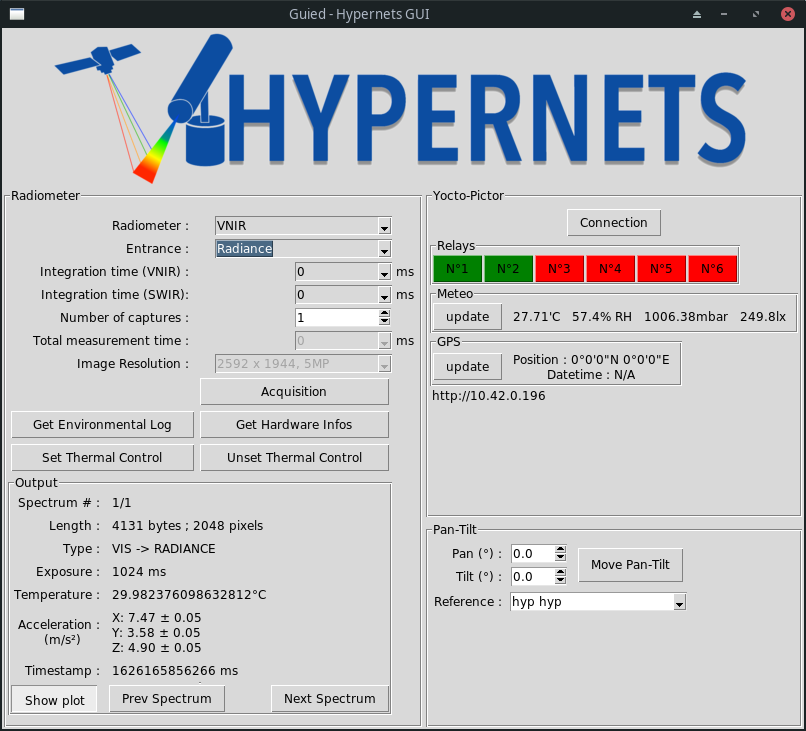
\includegraphics[width=\linewidth]{images/gui_overall.png}
% 	  \vspace{11pt}
% 	  \caption{Graphical User Interface}
% 	\label{fig:gui}
%   \end{minipage}
%   \hfill
%   \begin{minipage}[b]{0.48\textwidth}
% 	  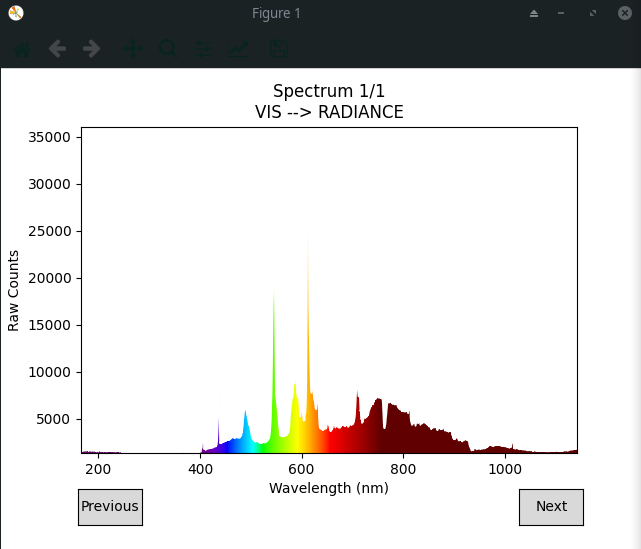
\includegraphics[width=\linewidth]{images/gui_graph.png}
% 	\caption{A Spectrum Plot}
% 	\label{fig:spectrumPlot}
%   \end{minipage}
% \end{figure}

\begin{figure}[!ht]
  \centering
  \begin{minipage}[b]{0.48\textwidth}
	  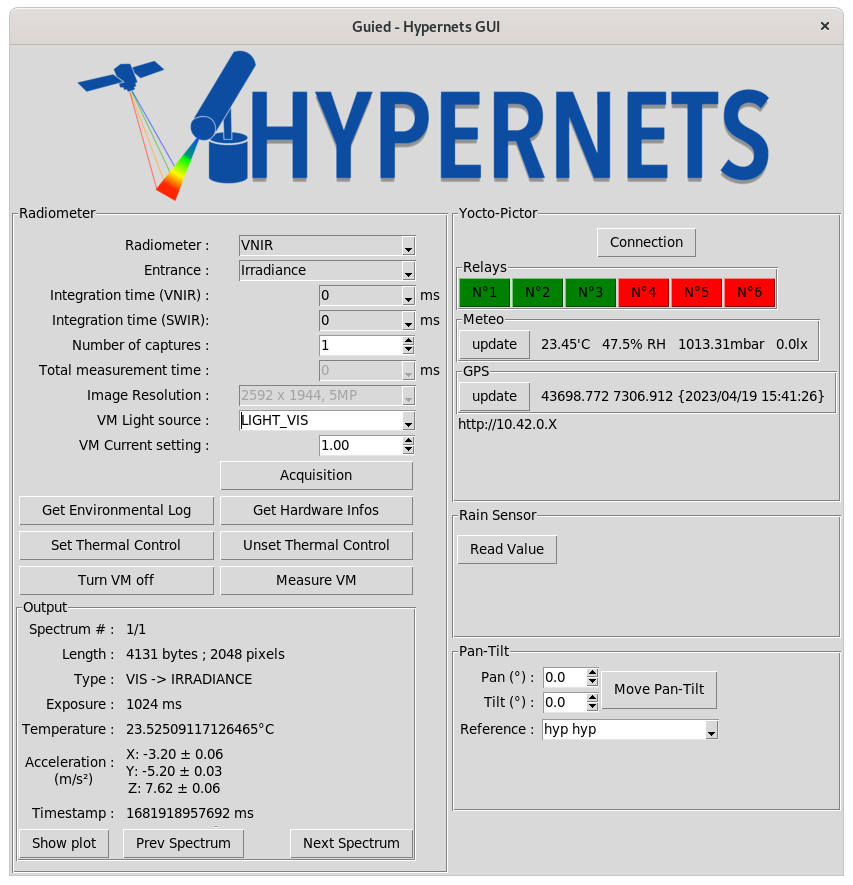
\includegraphics[width=\linewidth]{images/gui_main.png}
	  \vspace{11pt}
	\vspace{-15pt}
	  \caption{Graphical User Interface}
	\label{fig:gui}
  \end{minipage}
  \hfill
  \begin{minipage}[b]{0.48\textwidth}
	  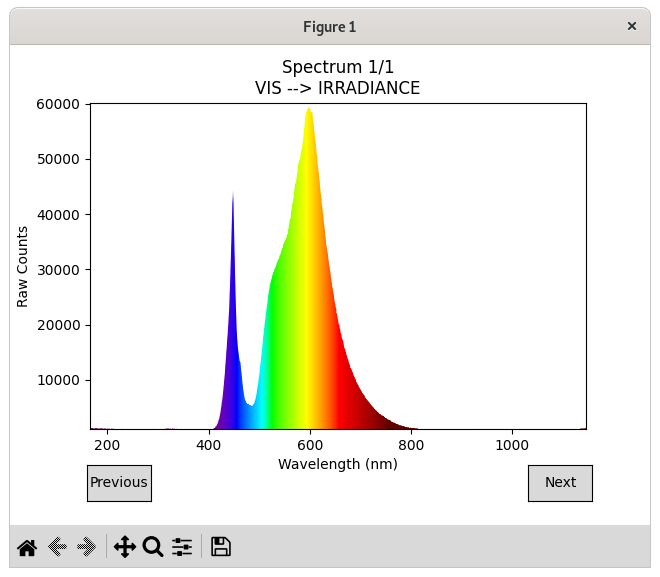
\includegraphics[width=\linewidth]{images/gui_spectrum.png}
	\vspace{-15pt}
	\caption{A Spectrum Plot}
	\label{fig:spectrumPlot}
  \end{minipage}
	\vspace{15pt}
	\vspace{15pt}
	\vspace{15pt}
  \begin{minipage}[b]{\textwidth}
	  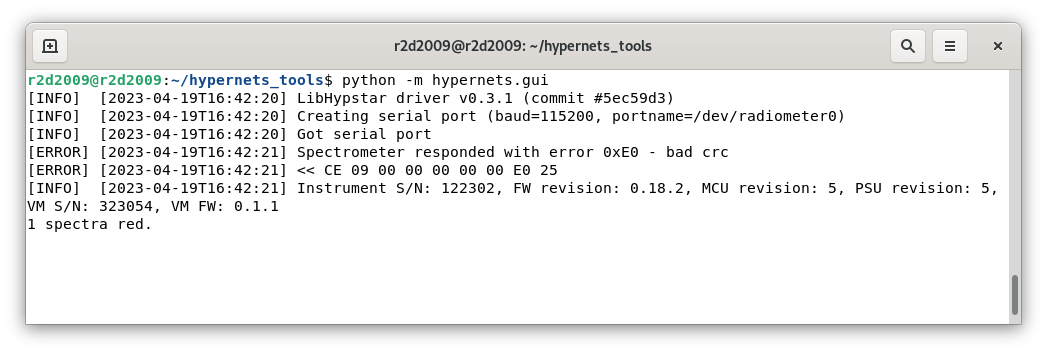
\includegraphics[width=\linewidth]{images/gui_console.png}
	\vspace{-15pt}
	\caption{Some Outputs on the console}
	\label{fig:spectrumPlot}
  \end{minipage}
\end{figure}

\clearpage
\newpage


\section{Autonomous System Mode}
% \subsection{Protocol Definitions}
% \subsubsection{Protocol v1}
% \subsubsection{Protocol v2}

\subsection{Set Relay n°1 ON at Wake-up}

Before using the studiel-box, we need to set the Yocto-Pictor first 
relay default value as ON. This aims to power-on the rugged-PC at the wake-up time
of the Yocto-Pictor. To achieve this, fire up a terminal and use those commands:
\begin{lstlisting}
cd hypernets_tools/
python -m hypernets.yocto.relay -fpon -n1
\end{lstlisting}

\noindent In order to test if it worked, hold the sleep button (the middle
one) on the Yocto-Pictor until it goes to sleep. Then wake it up by pressing 
the wake-up button (the upper one on the figure \ref{fig:yoctoSleep}). 
The relay 1 should be closed and the associated green LED (i.e. the LED 1 ; on the 
right of the card in the figure \ref{fig:yoctoSleep}) should light.

\begin{figure}[h!]
	\centering
	\cutpic{5pt}{.50\linewidth}{images/yoctopuce_sleepbutton.png}
	\caption{Yocto-Pictor: Three black buttons on the upper-left corner 
			 \& Green Relay Light on the right side of the bottom card}
	\label{fig:yoctoSleep}
\end{figure}
\FloatBarrier

\subsubsection{Enable SSH access}
Closing the Studiel-box will make our system \emph{headless}.
\emph{i.e.} it won't have any keyboard, screen or mouse connected on it. 
As we still need to interact  with it, a workaround solution is to connect to Wi-Fi 
and access it through a SSH, 
\emph{a Secure Shell}. To enable this service, type those two lines in terminal:
\begin{lstlisting}
sudo systemctl enable sshd    # For Manjaro 
sudo systemctl start sshd
sudo systemctl enable ssh    # For Debian 
sudo systemctl start ssh
\end{lstlisting}
Expected output:
\vspace{-10pt}
\begin{lstlisting}
Created symlink /etc/systemd/system/multi-user.target.wants [...]
\end{lstlisting}
Then, try to connect to the Wi-Fi with any laptop and SSH like this 
(you can use \href{https://www.putty.org/}{Putty} on Windows):
\begin{lstlisting}
ssh 'rugged_pc_user_name'@10.42.0.1
\end{lstlisting}

\subsection{Try a full sequence acquisition}
Now edit the \textit{dynamic configuration} file and edit it with the
following values:
\begin{itemize}
	% (see secion :\ref{})
	\item sequence\_file = \textit{path to the sequence of your choice} 
	\item start\_sequence = yes
	\item keep\_pc = on
\end{itemize}

Then, run the command below and see if it works. The output \textit{sequence
directory} should be saved in the folder \textit{DATA}. Its name is prefixed by
\textit{SEQ} and given according to the \textit{current UTC date and time} 
with the following format: \textit{SEQYYYYMMDDTHHMMSS}.
\begin{lstlisting}
./utils/run_service.sh
\end{lstlisting}
%After any modification of your config\_file.ini, you can try 
%this to check if it worked.
If everything is working properly, you can refer to the yoctopuce 
\href{https://www.yoctopuce.com/EN/products/yoctohub-wireless/doc/YHUBWLN1.usermanual.html#CHAP9SEC1}{wake-up scheduler documentation} 
in order to configure the system to wake up autonomously.
In addition, to enable the automatic run of the sequence every time the system
wakes up, run the installation script: 
\begin{lstlisting}
sudo install/04_setup_script_at_boot.sh
\end{lstlisting}

\subsection{Setup Server Communication}

If not already done, generate a ssh key with:
\begin{lstlisting}
ssh -t rsa
\end{lstlisting}

Edit the section \textit{network} of the file \textit{config\_static.ini}, 
create an empty directory in the appropriate folder on the server and run: 
\begin{lstlisting}
sudo install/05_setup_server_communication.sh
\end{lstlisting}

\textit{Example:} if your site name is 



% \FloatBarrier

% relays 2 and 3 and see if you are able to move the pan-tilt and take spectra.
% Annex on calibration offset pan-tilt and geometry.
% \FloatBarrier

% \subsubsection{(optional) Jupyter and Voilà! as a more user friendly access}


% \textcolor{red}{Draft!}: \href{https://jupyter.org}{Jupyter doc} and 
% \href{https://voila.readthedocs.io/en/stable/using.html}{voilà! presentation}.

% \newline

%% \begin{lstlisting}
% ./install/DD_install_jupyter.sh
% \end{lstlisting}
 
% \emph{Note that there is no sudo here.}
% Try then to connect with a webrowser to this address:
% \begin{lstlisting}
% https://10.42.0.1:8888
% \end{lstlisting}


%==============================================================================%

\section{Annexes}

\subsection{Configuration file: static\_config.ini}
\label{annex:staticconfig}

The \emph{static configuration file} is the file dealing with the parameters
that user will preferably not change. It includes the communication 
settings with the Yocto-Pictor and the server
credentials. As it contains critical settings, this file will not be 
automaticaly synchronized over the network.

\subsubsection{Section: yoctopuce}
\label{annex:configYocto}
\begin{tabularx}{\textwidth} {
        | >{\hsize=.15\hsize}X
        | >{\hsize=.6\hsize}X
		| >{\hsize=.25\hsize}X | }
	\hline
	\textbf{field} & \textbf{definition} & values (\textbf{default}) \\
	\hline
	\hline
	yoctopuce\_ip &	Yocto-Pictor-Wifi IP Address & 10.42.0.X
	\\ \hline
	yocto\_prefix1 & Yocto-Pictor Serial (relay board) & OBSVLFR1-XXXXXX
	\\ \hline
	yocto\_prefix2 & Yocto-Pictor-Wifi Serial &	OBSVLFR2-XXXXXX
	\\ \hline
	yocto\_gps & Yocto-GPS-V2 Serial & YGNSSMK2-XXXXXX
	\\ \hline
	bypass\_yocto & Bypass Yocto-Pictor during in a sequence (debug mode) & 
	\textbf{no} \\ \hline
\end{tabularx}

\subsubsection{Section: network}
\label{annex:configNetwork}

\begin{tabularx}{\textwidth} {
		| >{\hsize=.2\hsize}X
        | >{\hsize=.65\hsize}X
		| >{\hsize=.15\hsize}X | }
	\hline
	\textbf{field} & \textbf{definition} & \textbf{default} \\
	\hline
	\hline
	credentials & user account and server name & user@server 
	\\ \hline
	remote\_dir & name of the remote directory where data/config/logs are
	pushed & \texttildelow/XXYY 
	\\ \hline

	ssh\_port &	ssh port used to connect to the server & 22
	\\ \hline

	remote\_ssh\_port & ssh port used to connect from the server to the host
	system (use ssh -p 20213 rugged\_pc\_user@127.0.0.1 to connect)
	& 20213
	\\ \hline

\end{tabularx}

	%  webcam\_sky
	%  webcam\_site & credentials (user/pass) + IP address of the webcams & 
	%  USER:PASS\_1@ ip\_cam\_sky
	%  USER:PASS\_2@ ip\_cam\_site  & 
	%  see section \textcolor{red}{TODO} 
	%  & \\ \hline


\subsection{Configuration file : dynamic\_config.ini}
\label{annex:dynamicconfig}
The \emph{dynamic configuration file} is a communication tool allowing the
user to remotely change settings of the system. Unlike the \emph{static
configuration file}, it is synchronized with an identical file on the server side.
Synchronization over the network is performed using the one with the more recent 
modification.

\subsubsection{Section: general}
\begin{tabularx}{\textwidth} {
        | >{\hsize=.15\hsize}X
        | >{\hsize=.65\hsize}X
		| >{\hsize=.2\hsize}X | }
	\hline
	\textbf{field} & \textbf{definition} & values (\textbf{default}) \\
	\hline
	\hline
	keep\_pc & state of the system at the end of the sequence & on / \textbf{off} 
	\\ \hline

	start\_sequence & start or no the sequence every time the system is turned 
	on & \textbf{yes} / no 
	\\ \hline

	auto\_update & check for update at start-up & yes / \textbf{no}
	\\ \hline

	sequence\_file 	& which protocol file to follow & \textit{path to file}
	\\ \hline
\end{tabularx}

\subsubsection{Section: GPS}
\begin{tabularx}{\textwidth} {
        | >{\hsize=.15\hsize}X
		| >{\hsize=.85\hsize}X| }
	\hline
	\textbf{field} & \textbf{definition} \\
	\hline
	\hline
	latitude  &  Cartesian latitude of the location (float)
	\\ \hline
	longitude & Cartesian longitude of the location (float)
	\\ \hline
\end{tabularx}


\subsubsection{Section: pantilt}
\begin{tabularx}{\textwidth} {
        | >{\hsize=.15\hsize}X
        | >{\hsize=.6\hsize}X
		| >{\hsize=.25\hsize}X | }
	\hline
	\textbf{field} & \textbf{definition} & values (\textbf{default}) \\
	\hline
	\hline
	offset\_pan    & Azimuth adjustement value (in degrees) to point to South or North & 
	[0 - 360] \textbf{0} \\ \hline
	offset\_tilt   & Zenith adjustement value (in degrees) to point to point
	the Nadir &
	[0 - 360] \textbf{60} \\ \hline
	reverse\_tilt & Change the sign of both Azimuth and Zenith &
	yes / \textbf{no} \\
\hline
\end{tabularx}


\subsubsection{Section: metadata}
Metadatas are the information embedded in each Hypernets Sequence folder. 
In particular, each metadata file will have \emph{a header}, that is, 
the top the file. This header contains some dynamic informations like 
the current date and time as well as static ones, for instance the site
identification. This section of the \emph{dynamic config file} is the 
exact content of each metadata header. Fields between brackets will be
automatically processed by the host system.

\begin{table}[H]
	\centering
	\begin{tabularx}{\textwidth} {
	        | >{\hsize=.25\hsize}X
	        | >{\hsize=.50\hsize}X
			| >{\hsize=.25\hsize}X | }
		\hline
		\textbf{field} & \textbf{definition} & values  \\
		\hline
		\hline

		principal\_invesigator & Name of the PI, & 
		\textit{Investigator name} 
		\\ \hline

		datetime & UTC date and time at the sequence start time (no need to edit) 
		& \{datetime\} \\ \hline

		hypstar\_sn &  Hypstar Serial Number  & 123456\\ \hline
		site\_id & A site ID with the naming convention: XXYY such as: \newline
			-- XX: two first letters of the site name  \newline
			-- YY two first letters of the country partners-name 
		& XXYY \\ \hline

		protocol\_file\_name & Self-reference to the \textit{protocol file name} 
		from the \textit{general section} of this file (no need to edit) &  
		\$\{general:sequence\_file\} 
		\\\hline

		latitude & Self-reference to the latitude from the GPS section of this file 
		(no need to edit) & \$\{GPS:latitude\} \\ \hline

		longitude & Self-reference to the longitude from the GPS section of this file 
		(no need to edit) & \$\{GPS:longitude\}\\ \hline

		offset\_pan\ & Self-reference to the \textit{protocol file name} 
		from the \textit{pantilt} of this file (no need to edit) &  
		\$\{pantilt:offset\_pan\} 
		\\\hline

		offset\_tilt\ & Self-reference to the \textit{protocol file name} 
		from the \textit{pantilt} of this file (no need to edit) &  
		\$\{pantilt:offset\_tilt\} 
		\\\hline

		offset\_tilt\ & Self-reference to the \textit{protocol file name} 
		from the \textit{pantilt} of this file (no need to edit) &  
		\$\{pantilt:offset\_tilt\} 
		\\\hline

		azimuth\_switch\ & Self-reference to the \textit{protocol file name} 
		from the \textit{pantilt} of this file (no need to edit) &  
		\$\{pantilt:azimuth\_switch\} 
		\\\hline

	\end{tabularx}
\end{table}
\noindent\textbf{Note :} if you want to see what your metadata header will look like,
you can use this command :
\vspace{-10pt}
\begin{lstlisting}
python -m hypernets.abstract.create_metadata
\end{lstlisting}

\subsubsection{Section: hypstar}

\begin{table}[H]
	\centering
	\begin{tabularx}{\textwidth} {
			| >{\hsize=.15\hsize}X
			| >{\hsize=.55\hsize}X
			| >{\hsize=.30\hsize}X | }
		\hline
		\textbf{field} & \textbf{definition} & values (\textbf{default}) \\
		\hline
		\hline
		hypstar\_port & path to the hypstar \textit{device file} 
		& \textbf{/dev/radiometer0} \newline
		/dev/ttyUSB5 
		\\ \hline
		baudrate & speed communication (in bauds) with the instrument 
		& \textbf{115200}, 460800, 921600, 3000000, 6000000, 8000000
		\\ \hline
		loglevel & Set the log verbosity of the communication with the instrument 
		& \textbf{ERROR}, INFO, DEBUG, TRACE 
		\\ \hline
		swir\_tec & Thermoelectric Cooler setting point (in degree Celsius) 
		the SWIR module
		& [ -15 ; +40 ] \textbf{0}
		\\ \hline
	\end{tabularx}
\end{table}


\begin{table}[H]
	\centering
	\begin{tabularx}{\textwidth} {
			| >{\hsize=.2\hsize}X
			| >{\hsize=.8\hsize}X|}
		\hline
		\textbf{Log Level} & \textbf{Definition}  \\
		\hline
		\hline
		ERROR & only errors are reported on stderr \\ \hline
		INFO & stdout + stderr \\ \hline
		DEBUG & driver command execution printout to stdout \\ \hline
		TRACE & low level communication bytes are printed to stdout \\
		\hline
	\end{tabularx}
\end{table}

%\begin{sidewaystable}
% Webcams: see this
% \href{https://github.com/HYPERNETS/hypernets\_tools/issues/35}{github issue}.
%\end{sidewaystable}

\subsection{How To Access to the BIOS of the Cincoze}
\label{annex:bios}
You will need to access to the \emph{Basic Input Ouput System} menu
(or BIOS CMOS Setup Utility) to perform some configuration tasks
like set-up the serial port or boot from USB stick. 
To get this acces, turn \emph{OFF} and \emph{ON} the computer, then immediately 
press \textbf{\textless del\textgreater} 
or \textbf{\textless ESC\textgreater}.
You should see a screen similar to the figure
\ref{screen_bios}. If not, you may refer to the
\href{http://www.cincoze.com/data/files/201509/Manual\_DE-1000\_R1.3\_20170621001.pdf}
{User's Manual of the computer}.
\vspace{11pt}

\begin{figure}[!h]
\centering
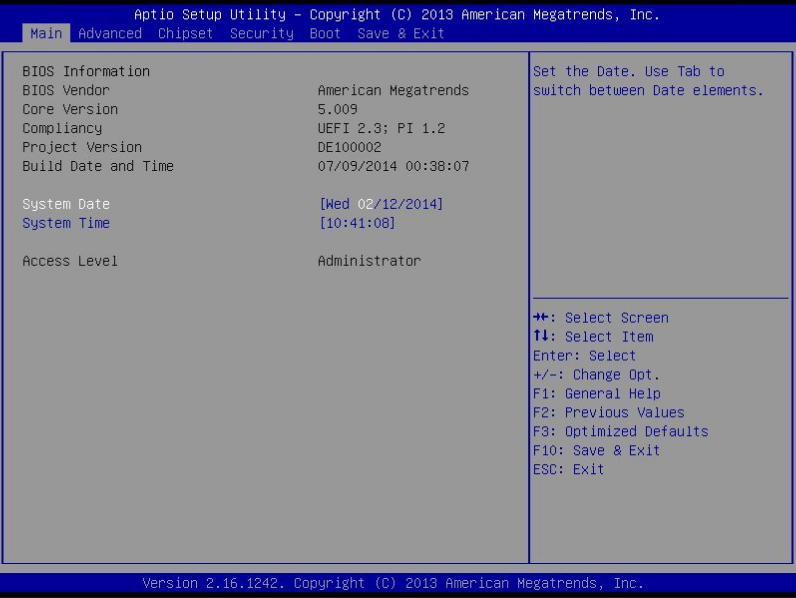
\includegraphics[scale=.43]{images/bios_screenshot.png}
\caption{Screenshot of BIOS}
\label{screen_bios}
\end{figure}

\subsubsection{Pan-Tilt: Serial Port Configuration}
Go to the BIOS (see annex \ref{annex:bios}). Under the tab \emph{Advanced}
go to the menu \emph{Super IO Configuration}, select the serial port for the 
pan-tilt (usually the n°4) and select \emph{RS485 Half Duplex} on the line 
\emph{Onboard Serial Port 4 Mode}. Save and exit. 


\subsection{Yoctopuce Tips}

\subsubsection{Upgrade Yocto-Pictor firmwares}
\label{annex:yoctoUpdate} 

Please refer to the
\href{https://www.yoctopuce.com/EN/products/virtualhub/doc/VIRTHUB0.usermanual.html#CHAP3SEC4}
{yoctopuce documentation} in order to upgrade the firmwares.

% TODO:
% Note : the yoctopuce has to be powered by external source using input socket not usb
% screen yoctoUpdate.zip 

\subsubsection{How to catch debug informations}

The Yocto-Pictor is still a tool under development and some bugs may
sometimes show up. So when something wrong happens. For example the software is 
reporting an error relative to yocto or the behaviour is not the one expected. 
It could be helpful to join a \emph{memory dump} of the card to the issue
report. In order to get this file, here is the most common scenario:

\begin{enumerate}
	\item Something goes wrong with the card.

	\item Don't touch anything but hold on the Ybutton during 5 seconds 
		(see figure \ref{fig:ybutton}).

	\item Now, restart the system in order to get back the Wi-Fi connection 
		working.

	\item Go to the yoctopuce webpage (by typing : 10.42.0.X:4444 in the
		address bar of a web browser).

	\item Click successively on \emph{Configure} (on the row of
		\emph{Yocto-Pictor-Wifi}), then \emph{manage files} 
		(see \ref{fig:fileman}).

	\item You should see a row with \emph{dump.bin} under the column
		\emph{Path/name}.
		Download this file, using \emph{right click} and \emph{Download
		Linked File}.
		(see \ref{fig:downloadDump}).

	\item Finally click on \emph{remove} to delete the file in order to avoid
		eventual future confusion.
\end{enumerate}

For convenience, you can name the file with your initials, the date and
an error reference if there is one. Also, please mind to always send this 
file with an explanation of the issue or the error logs.

\begin{figure}[H]
  \centering
  \begin{minipage}[b]{0.40\textwidth}
	  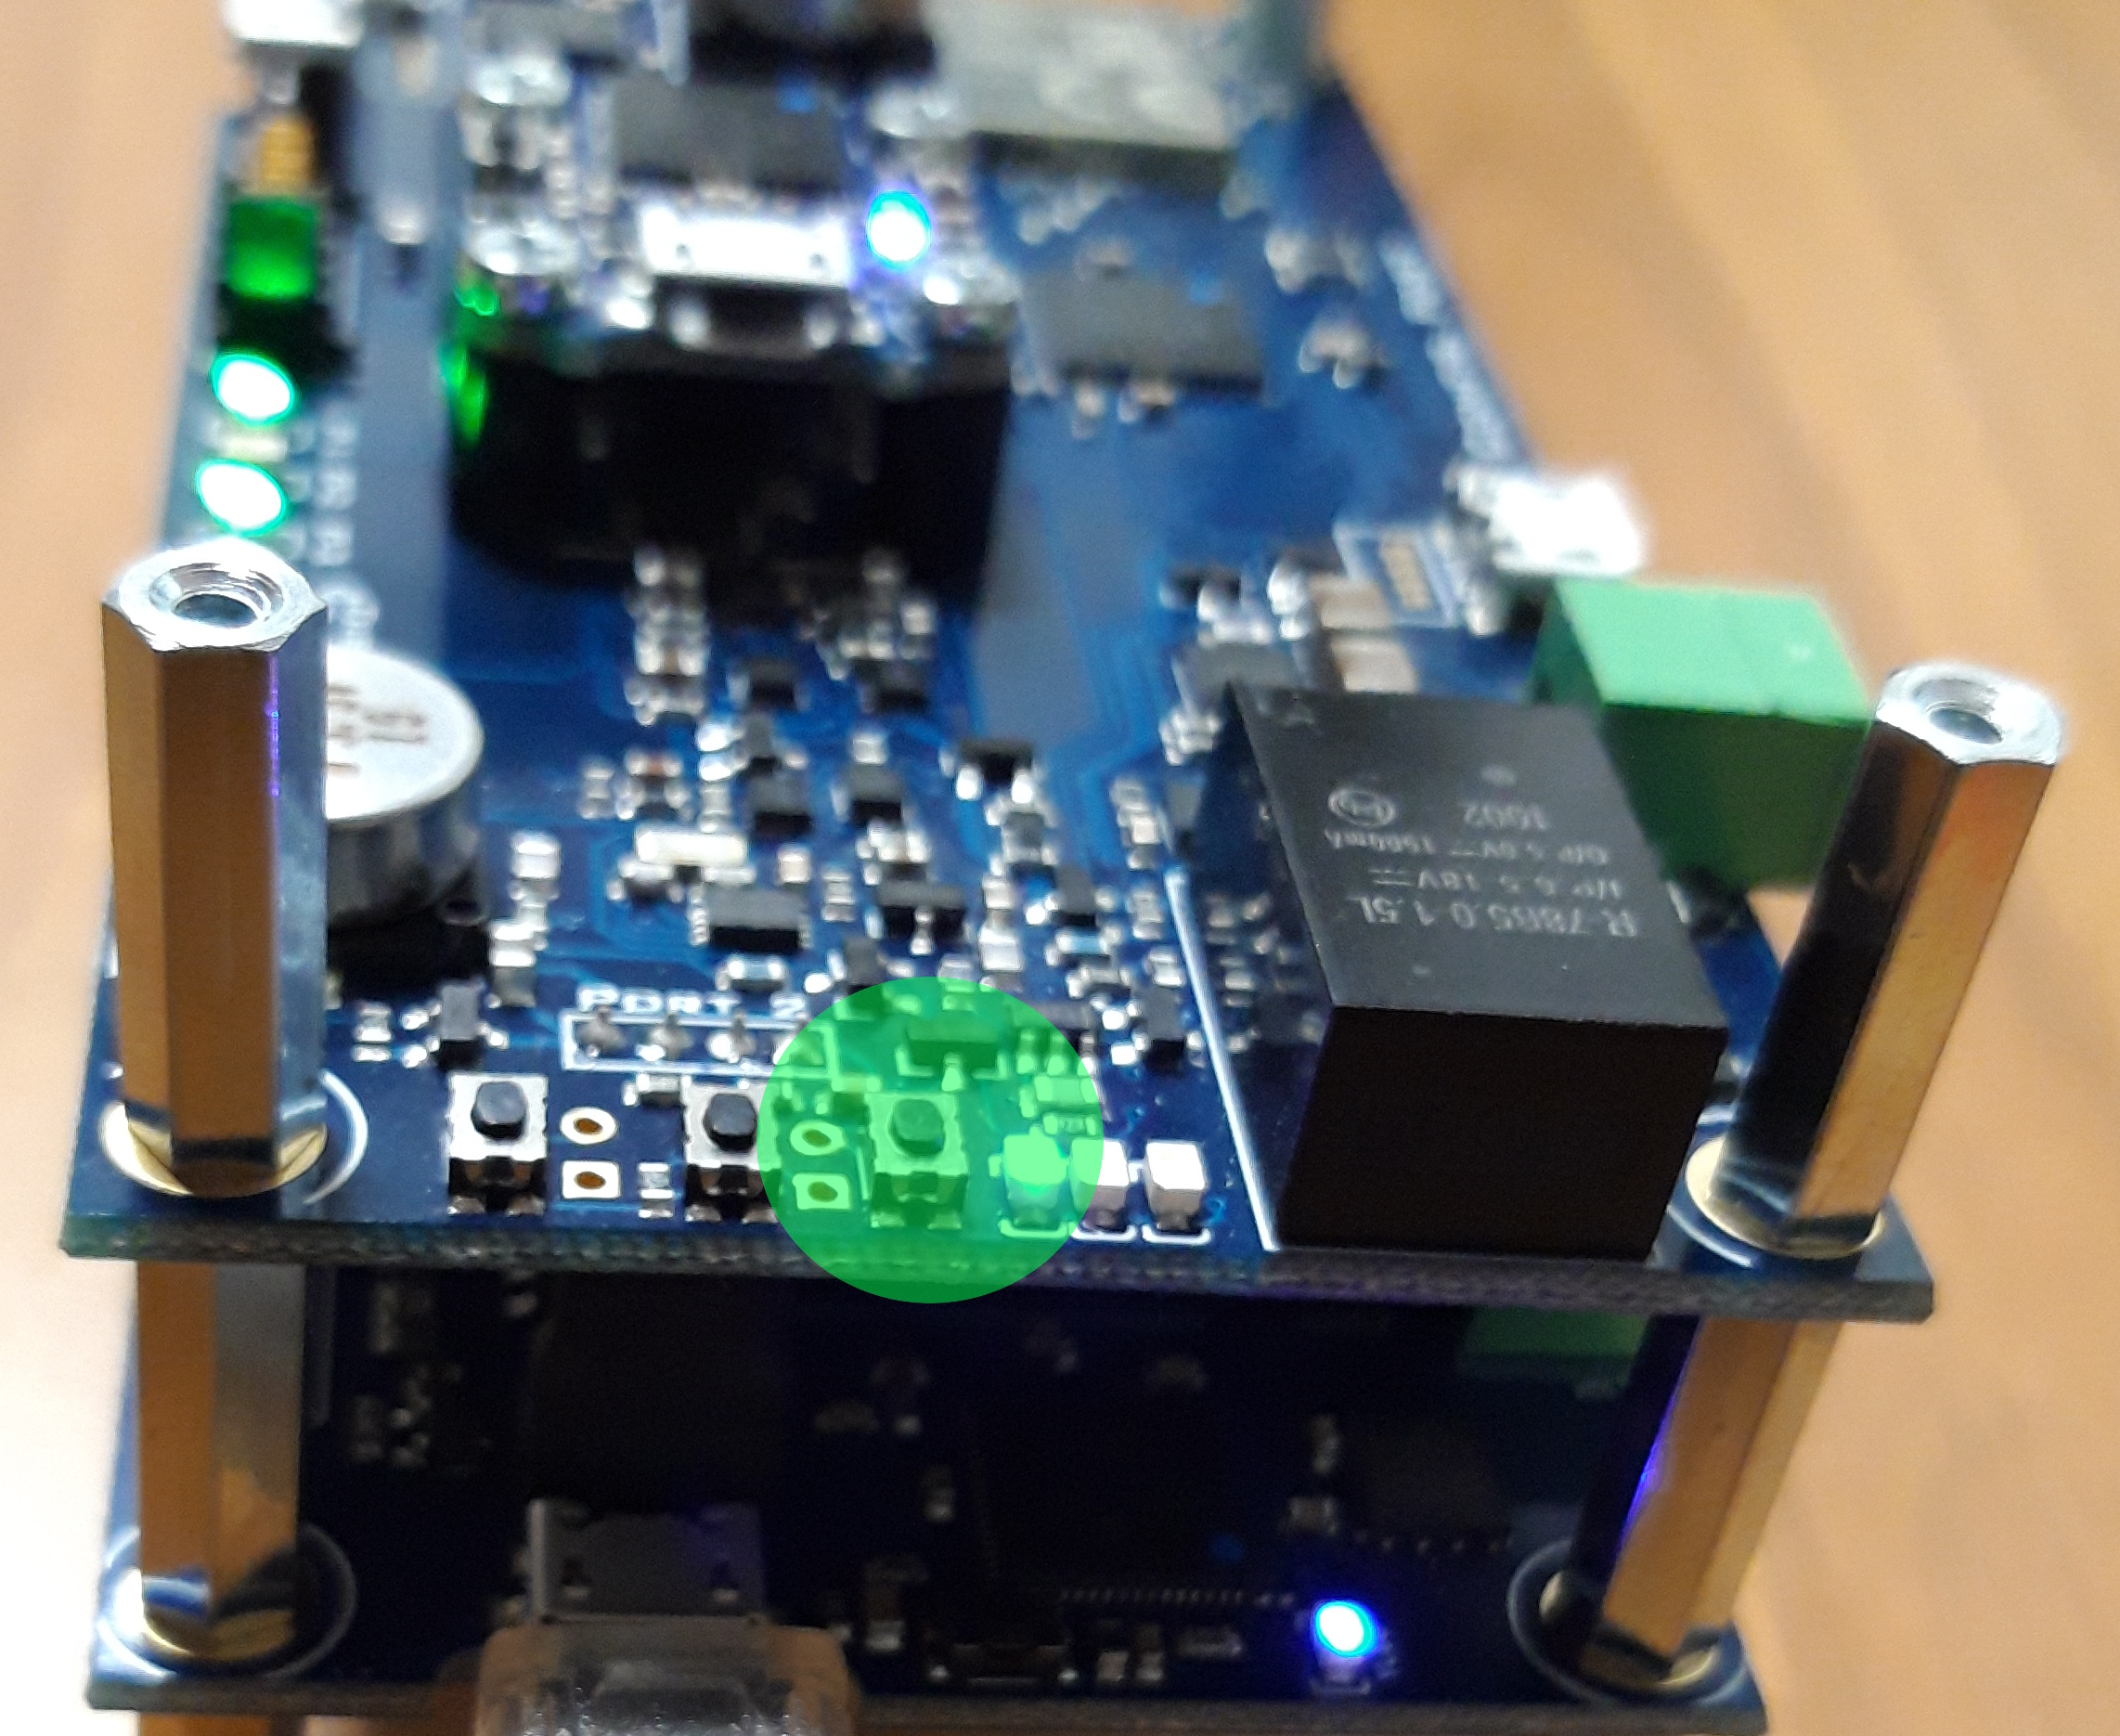
\includegraphics[scale=.09]{images/yoctopuce_bug1.jpg}
	  \caption{Highlighted \emph{YButton}}
	  \label{fig:ybutton}
  \end{minipage}
  \hfill
	\vspace{15pt}
  \begin{minipage}[b]{0.50\textwidth}
	  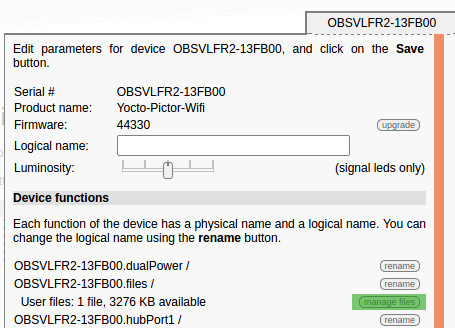
\includegraphics[scale=.54]{images/yoctopuce_bug2.jpg}
	  \caption{Hightlighted \emph{file manager}}
	  \label{fig:fileman}
  \end{minipage}
  \begin{minipage}[b]{0.50\textwidth}
	  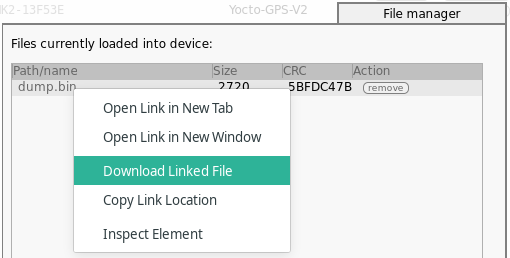
\includegraphics[scale=.54]{images/yoctopuce_bug3.png}
	  \caption{Download \emph{dump.bin}}
	  \label{fig:downloadDump}
  \end{minipage}
\end{figure}


%==============================================================================%
 -----------------------------------------------------------------------------%
%                            OLD VERSION MANUAL
% -----------------------------------------------------------------------------%

\section{Old Versions Documentation}


\subsection{Manjaro Linux System}

\subsubsection{Creating A Live USB Of Manjaro Linux}
\label{usbLiveCreation}
\par First, please go to 
\href{https://manjaro.org/downloads/official/xfce/}
{manjaro archive download page} and download the "minimal" version ISO of 
Manjaro linux 21.0.
Then, make the ISO file Bootable on USB drive. Under Windows, you
can do it by using \href{https://www.easy2boot.com}{easy2boot} for example. 
Under Linux and Mac, you can use the following instructions.
\newline
\par
Open a terminal, type the following command: 
\begin{lstlisting}[language=commandline]
sudo dmesg -w
\end{lstlisting}

Now connect your USB stick memory, you should get output similar to this:
\begin{lstlisting}[language=commandline, style=output]
[10576.130389] usb-storage 2-6:1.0: USB Mass Storage device detected
[10576.130756] scsi host5: usb-storage 2-6:1.0
[10577.144722] scsi 5:0:0:0: Direct-Access     SanDisk  Ultra USB 3.0    
1.00 PQ: 0 ANSI: 6
[10577.145229] sd 5:0:0:0: Attached scsi generic sg6 type 0
[10577.145493] sd 5:0:0:0: [sdf] 30031872 512-byte logical blocks: 
(15.4 GB/14.3 GiB)
[10577.146230] sd 5:0:0:0: [sdf] Write Protect is off
[10577.146233] sd 5:0:0:0: [sdf] Mode Sense: 43 00 00 00
[10577.146485] sd 5:0:0:0: [sdf] Write cache: disabled, read cache: 
enabled, doesn't support DPO or FUA
[10577.153805]  sdf: sdf1
[10577.155586] sd 5:0:0:0: [sdf] Attached SCSI removable disk
\end{lstlisting}

Here, the linux device naming for the USB key is \emph{/dev/sdf} (line 12).
Next step is to \emph{unmount} all file systems of this USB key from
the file hierarchy in order to prevent any access by other application.
Then we need to format the unmounted drive in Linux jounaling file system
\emph{ext4}.
And finally copy the Manjaro Linux ISO file to the USB drive.
Adapt the following commands with the name of your device and the path to the
ISO file you just downloaded. Note the ending star for the first command.

\vspace{6pt}
\textbf{\textcolor{red}{Warning: it is critically important not to copy the ISO onto the
wrong device! Please double check before going ahead with the next.}}

\begin{lstlisting}
umount /dev/sdf*
sudo dd if=/path/to/manjaro.iso of=/dev/sdf status="progress"
\end{lstlisting}
If ISO is properly copied to bootable USB, you should see the new name 
MJRO1815 for the USB key.

% -----------------------------------------------------------------------------%
\subsubsection{Install and Update Manjaro Linux}
Insert the Live USB flash drive into the computer, power it, and get access to the
BIOS (see annex \ref{annex:bios}). Go under the tab named \emph{Boot} and press enter 
on the menu \emph{Hard Drive BBS Priorities}. You should see the name of your hard-drive 
on the first row and the name of your usb drive on the second one. If you don't see your 
USB key in here this may mean your bootable USB key is not made properly.
Use \textbf{\textless+/-\textgreater} controls to put your flash drive on the first, 
then press \textbf{\textless Esc\textgreater} to quit the menu, go under 
\emph{Save \& Exit} and select \emph{Save Changes and Reset}.
% Note : BBS = BIOS Boot Specification
\newline
\par

\begin{minipage}[c]{0.15\textwidth}

\includegraphics[width=\textwidth]{images/manjaro0.png}
\end{minipage}
\hfill
\begin{minipage}[c]{0.75\textwidth}
Once Manjaro has started, double-click on the icon \emph{Install Manjaro Linux}
(lower left corner)
\begin{itemize}
	\item Use American English (US)
	\item Choose Europe as Region and London as Zone
	\item Choose ERASE DISK
	\item Login and password (use same for administrator)
\end{itemize}
\end{minipage}
\par
\vspace{11pt}
Then reboot again without the USB stick. After getting your desktop environment 
started, set up an Internet connection, open a terminal (press 
\textbf{\textless ctrl + alt + t \textgreater}) and type the following commands
in the terminal in order to clean your \textit{home directory} 
update the system and install \textit{git}:
\begin{lstlisting}
rmdir Music/ Pictures/ Videos/ Public/ Templates/
sudo pacman -Syu
sudo pacman -S git
sudo pacman -S git
\end{lstlisting}

\noindent Say yes/or default [ENTER] to all questions. Note that once done, the computer may 
reboot.

\clearpage

\subsection{Wi-Fi Connection Between the Yocto-Pictor and the rugged PC}
\timeclock{0}{10}
\vspace{16pt}

The Yocto-Pictor, provided as the electronic card of Hypernets system is
controlled through Wi-Fi by the rugged PC. The three following subsections
describe how to set-up this communication.

\subsubsection{Wi-Fi Hotspot Set-up}
\label{sec:wifirugged}
\par
This part aims to configure the Wi-Fi of the rugged PC. It will mainly be used
to control the Yocto-Pictor. But will also be useful to access the rugged PC
after having installed it in the main box of the system.

\begin{itemize}
	\item First, right click on the the connection logo in the bottom right corner of the
screen and click \emph{Edit Connections...} (see figure \ref{fig:editConnection}). 
	\item Click on  \textbf{+}  to add a new connection and select \emph{Wi-Fi} for the 
		Connection Type. 

		On the tab \emph{General}:
		\begin{itemize}
			\item Check \emph{Connect automatically with priority 1}
			\item Check \emph{All users may connect to this network}
		\end{itemize}

		On the tab \emph{Wi-Fi}:
		\begin{itemize}
			\item Set the mode to \emph{Hotspot}
			\item Choose a \emph{SSID}: the name that will appear as Wi-Fi network. 
		\end{itemize}

		On the tab \emph{Wi-Fi Security} (see figure \ref{fig:wifiConfig}).
		\begin{itemize}
			\item Set the security to \emph{WPA \& WPA2 Personal}, 
			\item Choose a valid password
		\end{itemize}
		\item Choose a connection name (on the very top)
		\item Save 
		\item Close the current window and finally left click on 
			the connection logo, \emph{Create New Wi-Fi Network} 
			(see figure \ref{fig:retrieveWifi})
			and select your connection in the drop-down list to enable it.
			
\end{itemize}


\textbf{Note:} further, you may want to use Wi-Fi connection to get an
internet acces. Keep in mind that you can switch the Wi-Fi connection and 
get back to the previous one by following this last step.


\begin{figure}[H]
	\centering
	\begin{minipage}[l]{0.49\linewidth}
		\centering
		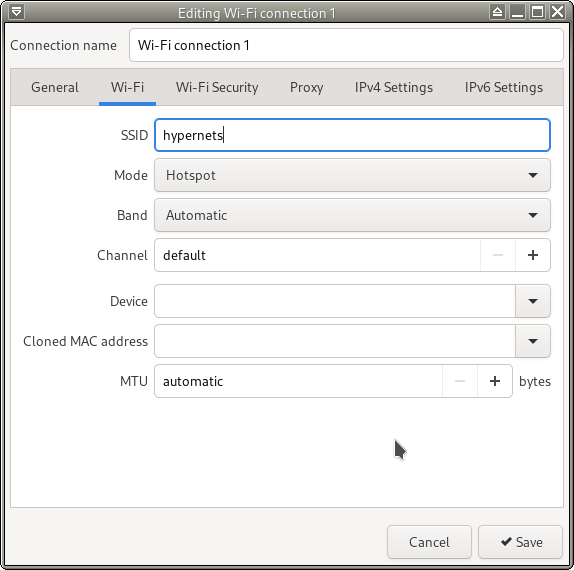
\includegraphics[width=\linewidth]{images/wifi2.png}
		\caption{Edit Connections}
		\label{fig:editConnection}
	\end{minipage}
	\begin{minipage}[r]{0.49\linewidth}
		\centering
		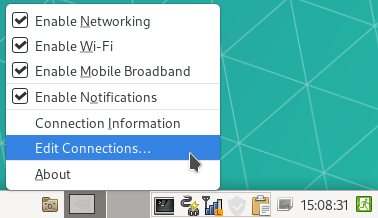
\includegraphics[width=.8\linewidth]{images/wifi1.png}
		\caption{Wi-Fi Connections Access}
		\label{fig:wifiConfig}
		\vspace{\baselineskip}
		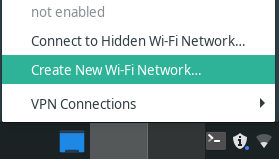
\includegraphics[width=.7\linewidth]{images/wifi3.png}
		\caption{Retrieve Wi-Fi Hotspot} \par
		\label{fig:retrieveWifi}
	\end{minipage}
\end{figure}


% -----------------------------------------------------------------------------%
\subsubsection{Setting up the Yoctopuce VirtualHub}
\label{sec:virtualhub}
% \timeclock{0}{10}
% \newline
\par 
According to the \href{https://www.yoctopuce.com/EN/virtualhub.php}{Yoctopuce
documentation}: 
\begin{quotation}
The VirtualHub is a toolbox for Yoctopuce USB devices. It will allow you
to:
	\begin{itemize}
	 \item configure and test Yoctopuce devices
	 \item remotely control Yoctopuce devices through network
	\end{itemize}
\end{quotation}

Here, you should have an updated linux distribution on your rugged PC and
a working internet connection wired on it.
Open a terminal, clone the installation script repository on your home folder,
and run the script with \emph{sudo priveleges}:

% git clone --recurse-submodules https://github.com/hypernets/hypernets_tools
\begin{lstlisting}
<ctrl + alt + t>  # open a terminal
cd
git clone https://github.com/hypernets/hypernets_tools
git checkout beta
cd hypernets_tools/
sudo ./install/00_install_yoctohub.sh
\end{lstlisting}
You should now be able to run the VirtualHub by typing:
\begin{lstlisting}
/usr/sbin/VirtualHub
\end{lstlisting}

% -----------------------------------------------------------------------------%
\subsubsection{Yocto-Pictor Wi-Fi Connection}
\label{sec:yocto-wifi}
\par
Run the VirtualHub (see last command in the previous section), 
open the web browser and visit the following address:
\begin{lstlisting}
127.0.0.1:4444
\end{lstlisting}
\par
If you don't see a screen like figure \ref{fig:screenyocto}, please retry 
instructions from the above section \pageref{sec:virtualhub}. 

If you were using Wi-Fi to get Internet, enable the hotspot (see last note from
section \pageref{sec:wifirugged})

Plug the Wi-Fi antenna (see figure \ref{fig:yoctoAntenna}) and connect the
Yocto-Pictor-Wifi with your usb cable on the config port (see figure \ref{fig:yoctoUSBtop}). 
Click on the button \emph{configure} and edit the \emph{WLAN settings} in the section 
\emph{Network Configuration}: 
\begin{enumerate}
		\item Select \emph{Infrastructure (choose an existing WLAN)}.
		\item Enter the password you choose in section \pageref{sec:wifirugged}.
		\item Click on \emph{Test Config} and note the displayed Current IP.
		\item Save and exit.
\end{enumerate}

Now, you can come back to your terminal with \textbf{\textless ctrl + alt + t \textgreater}
and quit the VirtualHub \textbf{\textless ctrl + c \textgreater}.

Type the IP address followed by \emph{":4444"} in the address bar of the web browser 
and you should see a screen similar to the one before with 3 lines and serials 
(see figure \ref{fig:yoctoSerial}). Note the 3 serials of these devices and the IP address. 
It will be required later (in the section \pageref{sec:yocto-config}).
\vspace{11pt}

\emph{Note: at this point you should consider to update the firmwares (see the
annex \ref{annex:yoctoUpdate})}

\begin{figure}[!ht]
  \centering
  \begin{minipage}[b]{0.35\textwidth}
	  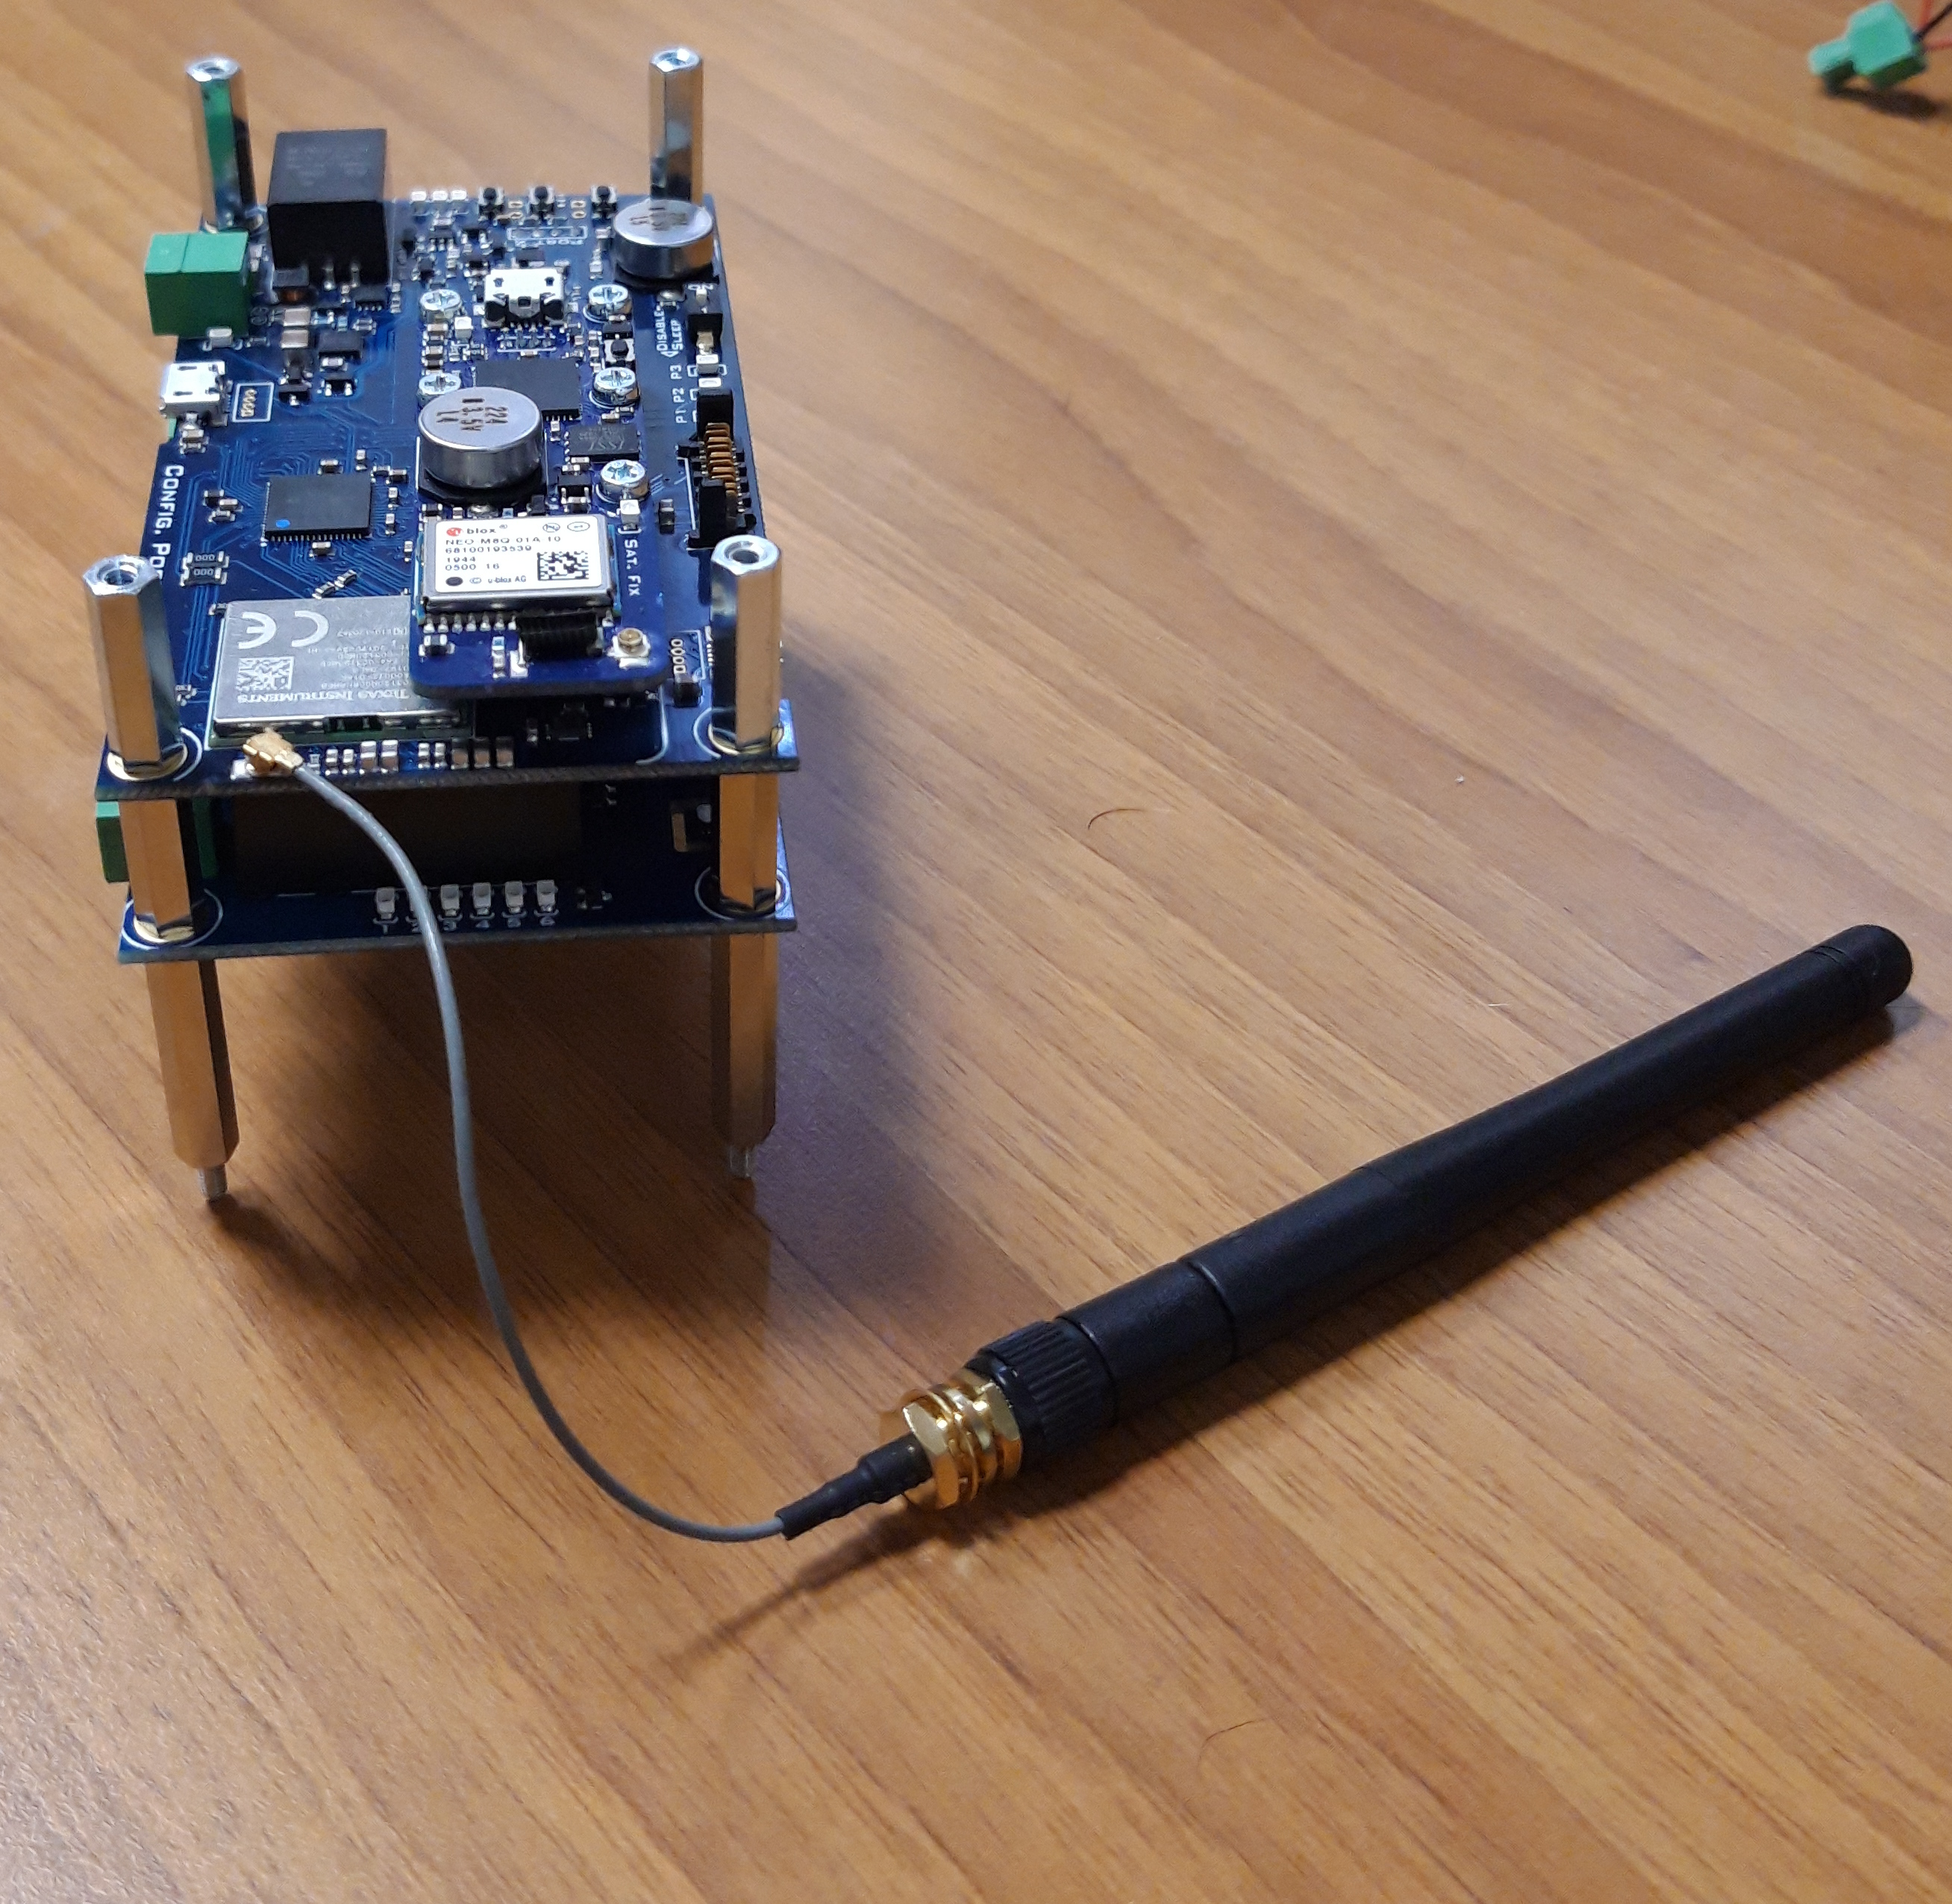
\includegraphics[width=\linewidth]{images/yoctopuce_wifi.jpg}
	\caption{Wi-Fi Antenna}
	\label{fig:yoctoAntenna}
  \end{minipage}
  \hfill
  \begin{minipage}[b]{0.55\textwidth}
	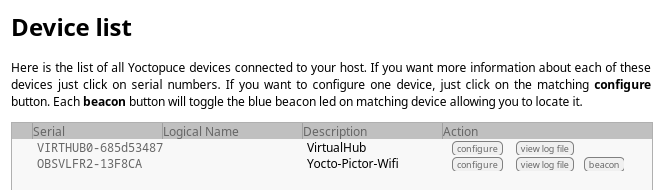
\includegraphics[width=\linewidth]{images/yocto1.png}
    \caption{Web Interface: Virtual Hub}
	\label{fig:screenyocto}
  \end{minipage}
\end{figure}

\begin{figure}[!ht]
  \centering
  \begin{minipage}[b]{0.35\textwidth}
	\includegraphics[width=\linewidth]{images/yoctopuce_usb2.jpg}
	  \vspace{11pt}
	\caption{Yocto-Pictor: top floor USB connection}
	\label{fig:yoctoUSBtop}
  \end{minipage}
  \hfill
  \begin{minipage}[b]{0.55\textwidth}
	  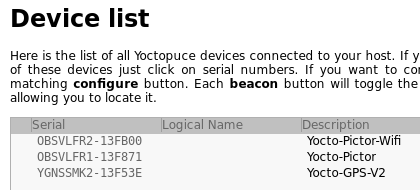
\includegraphics[width=\linewidth]{images/yocto3.png}
	\caption{Web Interface: serial}
	\label{fig:yoctoSerial}
  \end{minipage}
\end{figure}

\subsection{Linking Hypernets Tools to the Yocto-Pictor}

\label{sec:yocto-config}
If not already done, first copy the two configuration file templates in 
the hypernets\_tools folder:

\begin{lstlisting}
cd hypernets_tools/
cp hypernets/resources/config_dynamic.ini.template config_dynamic.ini
cp hypernets/resources/config_static.ini.template config_static.ini
\end{lstlisting}

Connect the PC to the internet, go to the folder \emph{hypernets\_tools} and 
install required dependencies:

\begin{lstlisting}
cd hypernets_tools/
sudo ./install/01_dependencies.sh
\end{lstlisting}

Now copy the template of the static configuration file 
(see description in annex \ref{annex:staticconfig}) and edit the Yoctopuce
section according to the serial that you previously noted in the section 
\pageref{sec:yocto-wifi}:

\begin{lstlisting}
cp hypernets/resources/static_config.ini.template static_config.ini
mousepad static_config.ini
\end{lstlisting}


If necessary, mind to switch back the Wi-Fi connection to the hotspot mode
(\ref{sec:wifirugged}) and try to run the Graphical User Interface (GUI) with: 

\begin{lstlisting}
python -m hypernets.gui.frame_yoctopuce
\end{lstlisting}

You should see some meteo and GPS data after clicking on \emph{Connection}. 
Also you can try playing with relays to check if everything is working 
(see figure \ref{gui_yocto}).


\begin{figure}[!ht]
	\centering
	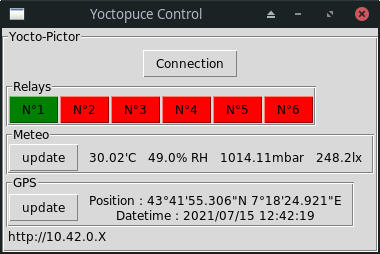
\includegraphics[scale=.55]{images/gui_yocto.png}
	\caption{GUI Yoctopuce Control}
	\label{gui_yocto}
\end{figure}


\subsubsection{Radiometer Configuration and First tests with the GUI}
\begin{itemize}
	\item Yocto-Pictor
	\item USB 2.0 cable of type A-micro B (data + power) 
\end{itemize}

Open a terminal and type the following command in order to link the radiometer
to a \textit{device file}:
\begin{lstlisting}
sudo ./install/02_configure_ports.sh
\end{lstlisting}
This should output with something like:
\begin{lstlisting}
lrwxrwxrwx 1 root root 7 Jul 15 15:04 /dev/radiometer0 -> ttyUSB5
\end{lstlisting}
Type the following command (required internet connection) to update the
\textit{libhypstar driver}:
\begin{lstlisting}
sudo ./install/03_update_libhypstar.sh
\end{lstlisting}


%==============================================================================%

\end{document}
